\chapter{Einleitung}
Das Domain-Name-System (DNS) bietet eine einfache Möglichkeit zur Namesauflösung und damit die Grundlage für menschenles- und merkbare Namen in modernen Computernetzwerken. Außerdem dient es als verteile Datenbank für simple Informationen über Netzwerke und Hosts. Speziell im Internet nimmt dieses Service damit eine zentrale Rolle im Verbindungsaufbau zwischen den vernetzen Systemen ein. Betrachtet man nun das Netzwerkprotokoll des DNS genauer, stellt man fest, dass es ohne jedliche Ansprüche an Informationssicherheit konzipiert wurde. Dieser Umstand ist dem Alter, beziehungsweise der Historie des Systems geschuldet, entspricht den heutigen IT-Sicheitsstandards jedoch in keinster weise. Aufgrund dieser Tatsache, wurden in den letzten Jahrzehnten verschiedenste Ansätze zur Lösung dieses Problems entwicket. Trotz dieses Umstands hat es bis zum heutigen Tag keiner der postulierten Standards geschafft eine weitreichende Durchdringung zu erlangen. Der gängige Weg DNS zu nutzen, hat sich, aus Sicht der Informationssicherheit, seit dessen Einführung nicht verändert.

% Grothoff Einbauen?

% Warum DNS Client? 

Diese Arbeit bietet eine kurze Einführung in die Funktionsweise von DNS (\ref{sec:DNS}) und gibt eine Übersicht der sicherheitsrelevanten Aspekten des Systems (\ref{sec:DNSSecurity}). Kern dieser Arbeit stellt eine Analyse der gängigsten Angriffsmethoden auf DNS-Clients, sowie deren Mitigation, dar (\ref{sec:Attacks}). Abschließend werden zwei konkrete Aufbauten beschrieben, die unter den Gesichtpunkten Sicherheit, Wirtschaftlichkeit und Wartbarkeit als optimal anzusehen sind. 
% TODO: Abschlussparagraph Nicht mehr ganz richtig

\section{Namensauflösung}
% Zu oberflächlich? Besser nur als Satz in DNS ?!

\section{DNS}
\label{sec:DNS}

DNS bietet ein Service zur standardisierten Auflösung von Ressourcennamen innerhalb globaler oder lokaler Computernetzwerke \cite{rfc1035}. Dabei werden menschenlesbare Zeichenketten (Namen) in Adressen übersetzt. Des Weiteren ist es möglich zusätzliche Informationen über diese Namen vom System abzufragen.

\subsection{Aufbau des DNS}

DNS ist als globale Datenbank mit Baumstruktur konzipiert, welche über eine beliebige Anzahl an vernetzten Rechern verteilt wird. Der Wurzelknoten wird als Root bezeichnet und wird von der Internet Assigned Numbers Authority (IANA), kontrolliert durch ein Komitee der \textit{Internet Corporation for Assigned Names and Numbers} (ICANN), betrieben. Die Daten dieses Wurzelknotens werden über 13 global verteilte Server bereitgestellt. Knoten der ersten Ebene werden als \textit{Top Level Domains} (TLDs) bezeichnet und sind nach Ländern (country-code TLD; ccTLD) oder Verwendung (genric TLD; gTLD). Manche Funktionen von DNS benötigen spezielle Domänen, welche unter einer eigenen Infrastruktur-TLD (.arpa) angelegt sind. Diese TLDs werden von verschiedenen Institutionen betrieben und stellen die höchste Stelle der DNS-Hirarchie dar und sind für die Weitergabe der Verwaltungsrechte für ihnen nachfolgende Domänen, sogenannte Second Level Domains (SLDs), verantwortlich. Die TLD .com wird, als Beispiel, von Verisign, Inc. betreut. Versign tritt somit als \textit{Registrar} der TLD .com auf. Will nun eine Person das Recht zur Verwaltung einer der .com Domäne nachgefolgten SLD erhalten, muss dies über einen Antrag bei dem Registrar, sprich Verisign, erfolgen. Ist die gewünschte Domäne, z.B. example.com, noch nicht vergeben, werden die Verwaltungsberechtigungen, gegen eine Gebühr, in den Besitz der/des Antragstellenden übergehen. Alle untergeordnenten Domänen sind damit ebenfalls in die Verantwortung übergegangen. Dieser Aufbau führt zu einer schichtweisen Delegation der Aufgaben innerhalb des globalen DNS-Namensraums (siehe Abb. \ref{img:dnsnamespace}). 

\begin{figure}[htbp]
    \centering
    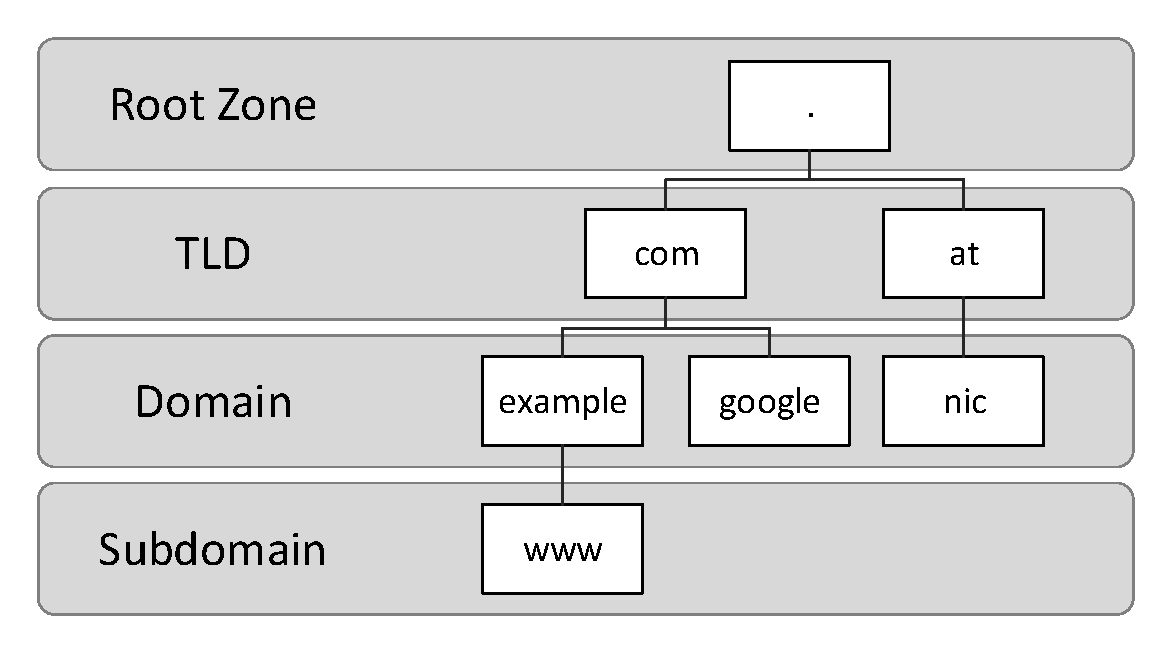
\includegraphics[width=\textwidth]{DNS_NameSpaceLayers}
    \caption{Aufbau des DNS}
    \label{img:dnsnamespace}
\end{figure}

\subsection{Ressource Records, Sets und Zonen}

Alle Datensätze in DNS werden in einer als \textit{Ressource Record} (RR) bezeichneter Datenstruktur abgelegt. Ein RR besteht dabei aus 5 Informationen: Namen, Time-To-Live (TTL), Klasse (Class), Typ (Type), Datenfeld (Data). Dabei sind die Felder TTL und Class optional. Die Menge an Einträgen mit gleichen Werten der Felder Name, TTL, Class und Type bilden dabei ein \textit{Ressource Record Set} (RRset) \cite{rfc2181}, das kleinstmögliche abfragbare Element in DNS. Alle RR die einem definierten, zusammenhängenden Teil des DNS Namensraum zugeordnet sind, werden als Zone bezeichnet. Diese Sammlung an RR wird in einem \textit{Zone File} gespeichert und von DNS-Server-Implementationen als Datenbasis genützt.   

Wie in Listing \ref{lst:dnsZoneFile} zu sehen ist, werden die Daten in einem menschenlesbaren Format gespeichert. Zeile 1 veranlasst das System zur Auflösung des Namens \textit{test.example.com.} zu den IPv4-Adressen \textit{172.30.0.7} und \textit{172.30.0.8}. Zeile 3 fügt dem Namen weiter Information im Freitextformat hinzu. Zeile 1 und 2 bilden zusammen ein RRset für \textit{test.example.com 3600 IN A}.

\begin{lstlisting}[caption={Ausschnitt aus dem Zone-File \textit{example.com}}, label={lst:dnsZoneFile}]
test.example.com.  3600  IN  A       172.30.0.7
                         IN  A       172.30.0.8
                         IN  TXT     "Text"
example.com.       1800  IN  MX      10 test.example.com.
example.com.       1800      NS      nameserver.example.org.
nameserver               IN  A       172.30.0.2
                         IN  AAAA    2001:db8:10::2
\end{lstlisting}

\subsection{DNS Server}

Um die globale, verteilte Datenbank des DNS nutzen zu können, ist es notwendig, dass diese den DNS-Client-Programmen zugänglich gemacht wird. Das Netzwerkprotokoll ist nach dem klassischen Client-/Server-Konzept ausgestaltet. Es erfordert keinen Verbindungsaufbau und verwendet einen einfachen, sequenziellen Ablauf an Anfragen und Antworten. Ein Client stellt dabei immer nur Anfragen an Server und verarbeitet deren Antwort. DNS-Server können hingegen, je nach Typ, auch selbst Anfragen an andere Server stellen und sind somit nicht nur auf das Beantworten von Anfragen beschränkt. Es können folgende DNS-Server-Typen unterschieden werden.

Die Software, die auf jedem Client-Rechner DNS-Anfragen von Programmen entgegennimmt und diese an die DNS Infrastruktur zur Auflösung übergibt, werden als \textbf{Stub resolver} bezeichnet. Diese können nach außen ausschließlich mit \textit{rekursiven Resolvern} kommunizieren und nehmen selbst keine Form der Namensauflösung vor. In manchen Fällen verfügen sie jedoch über einen Cache oder können aufgrund lokaler Policies (z.B. einem Hosts-File) eine Namensauflösung auf anderem Wege durchführen.

\textbf{Rekursive Resolver} (recursive Resolver) sind spezielle DNS-Server die von Clients genützt werden um Namen aufzulösen. Sie verfügen meistens über keine eigenen Zonen und sind damit als Vermittlungskomponente zwischen Endgeräten und den im Internet verfügbaren DNS-Servern zu verstehen.

Server deren Hauptaufgaben im Auflösen von Namen einer oder mehrerer bestimmter Zonen besteht, werden \textbf{authoritative Server} genannt. Die Bezeichnung spiel auf den Umstand an, dass die Antworten dieses Servers die finale Wahrheit über die von ihm verwalteten Zonen darstellt. Sie lesen die Antworten also direkt auf dem Zonen-File der entsprechenden Zone und verlassen sich nicht auf Antworten anderer Server oder Caches. Authoritative DNS-Server stellen damit die Endpunkte der Auflösung für die jeweiligen Domänen dar.

Eine spezielle Form des \textit{Rekursive Resolver} wird als \textbf{Forwarding DNS Server} bezeichnet. Aus Sicht des Stub Resolvers wirkt es wie ein gewöhnlicher Rekursiver Resolver. Der Unterschied besteht darin, dass er selbst keinen Auflöseprozess durchführt sondern die Anfragen lediglich an einen anderen Server weiterleitet, welche dann die eigentliche Auflösung durchführen. Die Ergebnisse werden meist gecacht und an den Client weitergegeben. 

\subsection{DNS Namensauflösungsprozess}

Der Namensauflösungsprozess erfolgt über mehrere Schritte und kann am besten anhand eines Beispiels dargestellt werden. Nehmen wir an, eine Applikation möchte die IPv4-Adresse des Namen exampe.com herausfinden und stellt eine Anfrage an den lokalen Stub Resolver (kurz stub) des Client. Folgende Schritte zusammen mit Abb. \ref{img:dnsresolution} erläutern den Prozess: 

\begin{enumerate}
    \item Der stub stellt eine Anfrage nach dem Type A Record der Domäne example.com an den für ihn konfigurierten rekursiven Resolver.
    \item Der resolver empfängt die Anfrage und prüft seinen lokalen Cache nach dem Eintrag. Da er diesen nicht aufgefunden wird fortgefahren.
    \item Nun startet der resolven den rekursiven Auflösungsvorgang. Geht man von einem leeren Cache aus, wird mit der Root-Zone (.) begonnen. Die Anfrage nach www.example.com wird dafür an einen der 13 vorkonfigurierten Root-DNS-Server gesendet.
    \item Der Root-Server empfängt die Anfrage, kann jedoch nur den TLD Teil der Antwort auflösen. Es sendet daher die Adressen des authoritativen Nameserver für die TLD .com zurück.
    \item Der Resolver verarbeitet nun die Adressen und sendet die Anfrage an einen der authoritativen Server der .com Domäne.
    \item Der TLD Nameserver empfängt die Anfrage und prüft, ob für die Domäne example.com eine entsprechende Deligation existiert. Da diese in Form mehrerer NS Einträge vorliegt, wird eine Liste an authoritativen Nameserver-Adressen der SLD Domäne example.com als Antwort gesendet.
    \item Da nun die Adresse eines authoritative Servers für die vollständige Zieldomäne example.com gefunden wurde, kann die gewünschte Information abgefragt werden. Der Resolver sendet also ein letztes mal die Anfrage des Client, jetzt an den Nameserver der SLD example.com.
    \item Der authoritative Server der SDL example.com nimmt die Anfrage nach dem RR mit Typ A für die Domäne example.com entgegen und liefert nun die gewünschte Information in Form einer IPv4 Adresse.
    \item Der rekursive Resolver empfängt die Antwort, überträgt sie in seinen Cache und sendet dem anfragenden stub die IPv4 Adresse zurück.
\end{enumerate}

\begin{figure}[htbp]
    \centering
    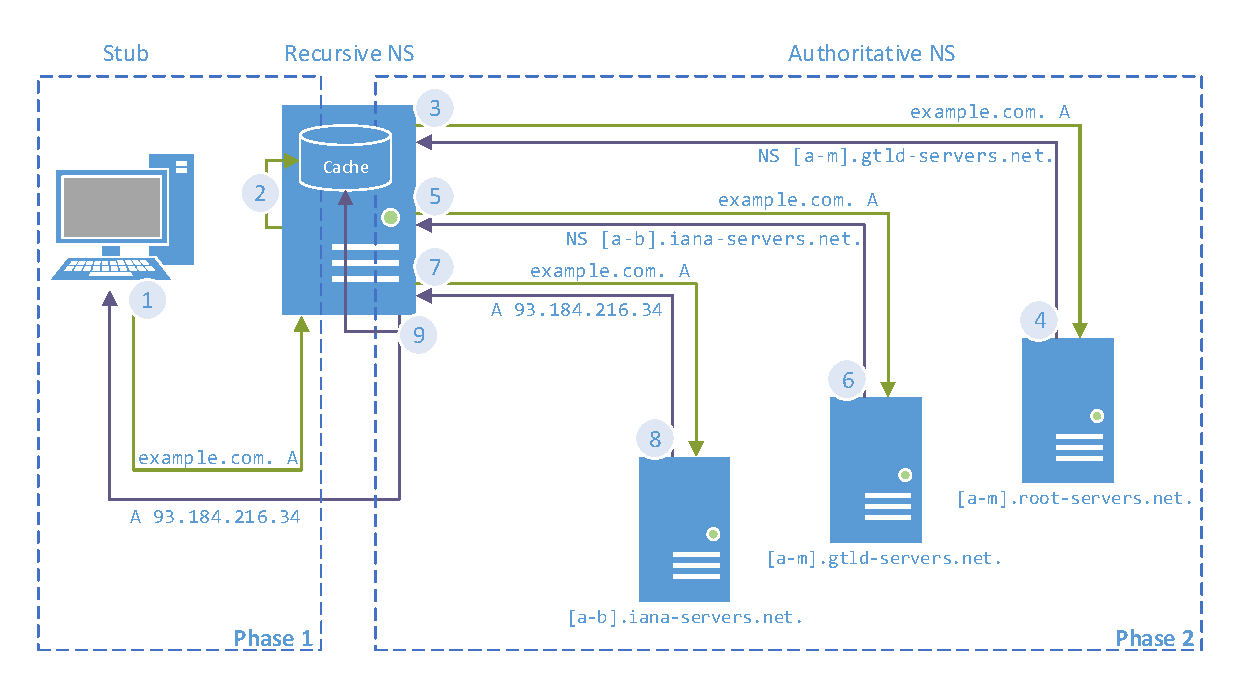
\includegraphics[width=\textwidth]{DNS_Resolution}
    \caption{Vollständiger Auflösungsprozess des Namen example.com über DNS }
    \label{img:dnsresolution}
\end{figure}

\section{DNS Security}
\label{sec:DNSSecurity}

Obwohl oder gerade weil DNS eines der grundlegendsten Protokolle im Internet darstellt wurde bei der Spezifikation des Netzwerkprotokolls bewusst auf eine Authentifizierung verzichtet. Dies ist auf die Idee einer öffentlich zugänglichen, globalen Datenbank, nach dem Vorbild eines globalen Telefonregisters, zurückzuführen. Die Datenbasis der Namensauflösung wurde somit als frei öffentlich zugänglich definiert. Außerdem stammt das Protokoll aus einer Zeit indem modernen Schutzzielen wie Sicherheit und Vertraulichkeit wenig Beachtung geschenkt wurde. Diese Umstände führten zu einer Vernachlässigung des Sicherheitsgedanken und hat sich über die Zeit zu einem ernstzunehmenden Problem entwickelt \cite{Grothoff2018}. Eine detaillierte Behandlung der Sicherheitsschwachstellen und der daraus resultierenden Bedrohungen ist den Kapiteln \ref{cap:weaknesses} und \ref{cap:threads} zu finden.

% Welche Probleme hat "klassisches" DNS? (Vertraulichkeit, Authentizität/Integrität)
% MitM (aLTEr, Crack, ARP-Poisoning, ...), Cache Poisoning, DNS Rebinding
% Transitiver Trust 

% Position des Resolvers

\chapter{Verwandte Arbeiten}

\lipsum

%DONT! JUST DONT! Wenn was streichen das das!